\chapter{Circuit Diagrams}
	
	This appendix contains the documentation required for the circuits produced
	within the project.
	
	\section{Control Electronics}
		\label{sec:mainboardDiagrams}
		
		The pinout for the Mbed (table \ref{tab:mbed}) and schematic
		(\ref{fig:electronics}) for the main board produced in the project are given
		below. The connections to stepper motors have been omitted for clarity (but
		the associated Mbed pins labelled).
		
		
		\begin{table}
			\centering
			\begin{tabular}{l l l l}
				\toprule
				Pin & Name & Definition & Connection \\
				\midrule
				1  & GND & & PSU Ground \\
				2  & VIN & & PSU +5V Standby \\
				3  & VB  & & Real-time Clock Battery (Unused) \\
				4  & nR  & & Reset switch \\
				5  & 5   & \verb|PIN_POWER_OK| & PSU Power OK \\
				6  & 6   & \verb|PIN_ENDSTOP_0_MIN|  & X-axis Min End-stop \\
				7  & 7   & \verb|PIN_ENDSTOP_0_MAX|  & X-axis Max End-stop \\
				8  & 8   & \verb|PIN_STEPPER_0_STEP| & X-axis Stepper Step \\
				9  & 9   & \verb|PIN_STEPPER_0_DIR|  & X-axis Stepper Direction \\
				10 & 10  & \verb|PIN_STEPPER_0_NEN|  & X-axis Stepper nEnable \\
				11 & 11  & \verb|PIN_ENDSTOP_1_MIN|  & Y-axis Min End-stop \\
				12 & 12  & \verb|PIN_ENDSTOP_1_MAX|  & Y-axis Max End-stop \\
				13 & 13  & \verb|PIN_STEPPER_1_STEP| & Y-axis Stepper Step \\
				14 & 14  & \verb|PIN_STEPPER_1_DIR|  & Y-axis Stepper Direction \\
				15 & 15  & \verb|PIN_STEPPER_1_NEN|  & Y-axis Stepper nEnable \\
				16 & 16  & \verb|PIN_ENDSTOP_2_MIN|  & Z-axis Min End-stop \\
				17 & 17  & \verb|PIN_ENDSTOP_2_MAX|  & Z-axis Max End-stop \\
				18 & 18  & & Unused \\
				19 & 19  & \verb|PIN_THERMISTOR_PLATFORM| & Platform Thermistor \\
				20 & 20  & \verb|PIN_THERMISTOR_EXTRUDER| & Extruder Thermistor \\
				\addlinespace
				21 & 21  & \verb|PIN_STEPPER_2_STEP| & Z-axis Stepper Step \\
				22 & 22  & \verb|PIN_STEPPER_2_DIR|  & Z-axis Stepper Direction \\
				23 & 23  & \verb|PIN_STEPPER_2_NEN|  & Z-axis Stepper nEnable \\
				24 & 24  & \verb|PIN_POWER_EN| & PSU Power On \\
				25 & 25  & & Unused \\
				26 & 26  & & Unused \\
				27 & 27  & \verb|PIN_HEATER_EXTRUDER| & Extruder Heater \\
				28 & 28  & \verb|PIN_HEATER_PLATFORM| & Platform Heater \\
				29 & 29  & \verb|PIN_EXTRUDER| & Extruder Motor \\
				30 & 30  & \verb|PIN_PLATFORM| & Platform Motor \\
				31 & D$+$  & & USB (Unused) \\
				32 & D$-$  & & USB (Unused) \\
				33 & TD$+$ & & MagJack (Ethernet) \\
				34 & TD$-$ & & MagJack (Ethernet) \\
				35 & RD$+$ & & MagJack (Ethernet) \\
				36 & RD$-$ & & MagJack (Ethernet) \\
				37 & IF$+$ & & Reserved (Unused) \\
				38 & IF$-$ & & Reserved (Unused) \\
				39 & VU    & & USB +5V (Unused) \\
				40 & VOUT  & & +3.3V Out \\
				\bottomrule
			\end{tabular}
			
			\caption{Mbed pin connections}
			\label{tab:mbed}
		\end{table}
			
		\begin{landscape}
			\begin{figure}
				\includegraphics[width=1.5\textheight]{circuits/electronics.pdf}
				\caption{Main board circuit diagram (direct connections to stepper controllers
				         omitted for clarity)}
				\label{fig:electronics}
			\end{figure}
		\end{landscape}
	
	\section{End-stop Electronics}
		
		The schematics and wiring colour codes for the end-stop electronics are
		given in this section.
		
		\subsection{Wiring Colour Codes}
			
			The colour codes for the connections from the end-stop board are given in
			table \ref{tab:endstopinterface} and the connections to the
			opto-interrupters are given in table \ref{tab:endstopoptoconnect}.
			
			\begin{table}[p]
				\centering
				\begin{tabular}{l l}
					\toprule
					Colour & Connection \\
					\midrule
					Green Solid    & Signal \\
					Green Striped  & Unused \\
					Blue Solid     & +5V \\
					Blue Striped   & +5V \\
					Orange Solid   & Unused \\
					Orange Striped & Unused \\
					Brown Solid    & Ground \\
					Brown Striped  & Ground \\
					\bottomrule
				\end{tabular}
				
				\caption{End-stop interface cat-5 wire allocations \cite{endstop}}
				\label{tab:endstopinterface}
			\end{table}
			
			\begin{table}[p]
				\centering
				\begin{tabular}{l l l l l}
					\toprule
					End-stop & LED $+$ & LED $-$ & Photo-transistor Collector & Photo-transistor Emitter \\
					\midrule
					X-axis     & Red    & Brown  & Orange & Yellow \\
					\addlinespace
					Y-axis min & Red    & Brown  & White  & Black  \\
					Y-axis max & Green  & Blue   & Orange & Yellow \\
					\addlinespace
					Z-axis     & Green  & Blue   & Purple & Gray   \\
					\bottomrule
				\end{tabular}
				
				\caption{Opto-interrupter connection colour codes}
				\label{tab:endstopoptoconnect}
			\end{table}
			
			
		\subsection{Schematic}
			
			\label{sec:endstopDiagram}
			
			The endstops are interfaced via the circuit in figure
			\ref{fig:endstopschem}. This circuit is duplicated once for each end-stop
			on the end-stop board.
			
			\begin{figure}[p]
				\center
				\includegraphics[width=0.5\textwidth]{circuits/endstop.pdf}
				\caption{End-stop circuit schematic.}
				\label{fig:endstopschem}
			\end{figure}
